\documentclass{beamer}
\setbeamertemplate{navigation symbols}{}

\usepackage{beamerthemeshadow}
\usepackage{graphicx}
\usepackage{url}
\usepackage{listings}

\begin{document}
\title{Stackbased Languages}
\author[Serap Kadam \and Christoph M{\"u}llner]{Serap Kadam \and Christoph M{\"u}llner \\
$<$serapkadam@gmail.com$>$, $<$christophm30@gmail.com$>$}
\subtitle{Knight's Tour}

\date{\today} 

\begin{frame}
\titlepage
\end{frame}

\begin{frame}
\frametitle{Table of contents}
\tableofcontents
\end{frame} 

\section{Knight's tour} 
\begin{frame}
\frametitle{The problem}
"The Knight's Tour is a mathematical problem involving a knight
on a chessboard. The knight is placed on the empty board and,
moving according to the rules of chess, must visit each square
exactly once. 

A knight's tour is called a closed tour if the
knight ends on a square attacking the square from which it began.
Otherwise the tour is open." from wikipedia 

In German this problem is called "Springerproblem".

\end{frame}

\subsection{Background}
\begin{frame}
\frametitle{The knight and his movement}
\begin{figure}
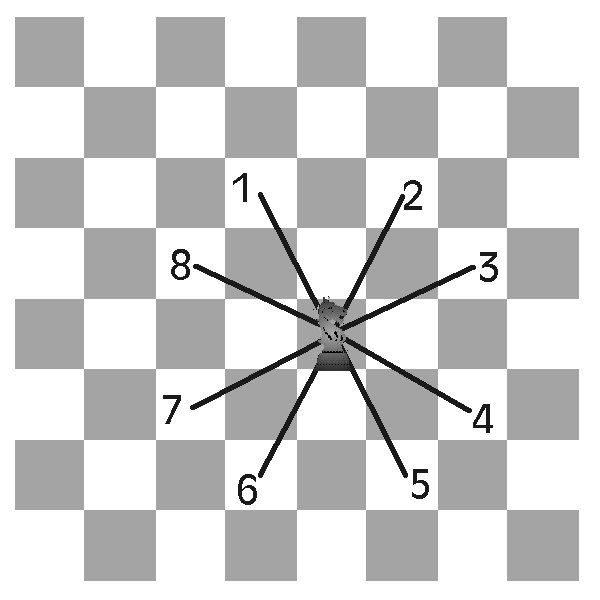
\includegraphics[scale=0.25]{sprung}
\caption{Possible moves of a knight}
\end{figure}
\end{frame}

\begin{frame}
\frametitle{One of many solutions}
\begin{figure}
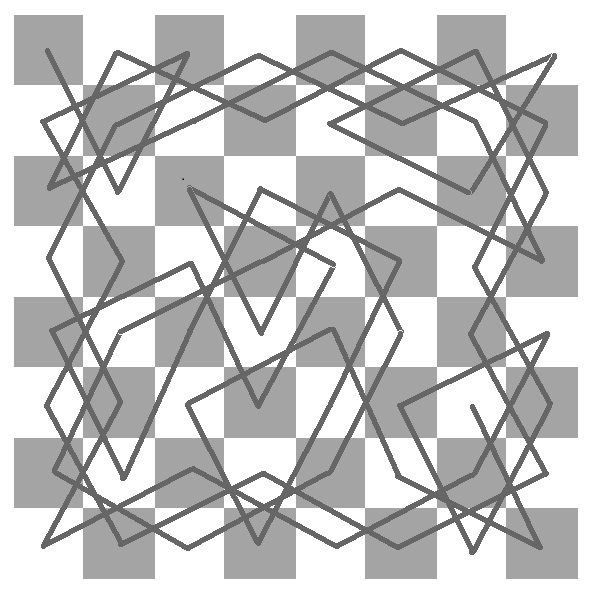
\includegraphics[scale=0.4]{loesung}
\caption{Possible solution on a $8x8$ chessboard}
\end{figure}
\end{frame}

\begin{frame}
\frametitle{An invalid solution}
\begin{figure}
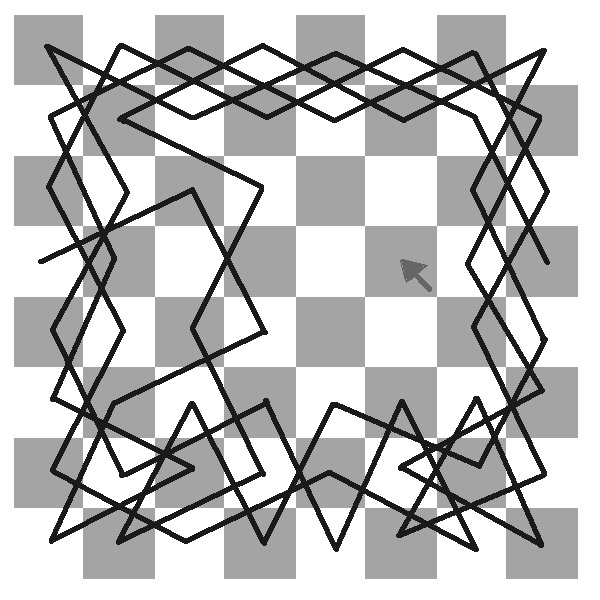
\includegraphics[scale=0.4]{luecke}
\caption{The marked square can't be reached anymore}
\end{figure}
\end{frame}

\begin{frame}
\frametitle{Warnsdorff's algorithm}
Heurisic by H. C. Warnsdorff (1823)\par
\begin{itemize}
	\item As long as there are reachable positions: visit unvisited position,
	which has the fewest successor positions
	\item Two positions with the same amount of successors $\rightarrow$
	choose* any of these positions
	\item Only a (very good) heuristic $\rightarrow$ must not find a solution
	\item Even with board size $8x8$ there might be no solution
\end{itemize}
*...Choosing the right value is very important.
\end{frame}

\section{Implementation}
\subsection{Language, task description}
\begin{frame}
\frametitle{Language}
\begin{itemize}
	\item Language: Forth (gforth)
	\item Used special language feature: data and return stack, factoring
\end{itemize}
\end{frame}

\subsection{Status and implementation details}
\begin{frame}
\frametitle{Algorithm}
\begin{enumerate}
	\item Start position on stack
	\item Lookup all neighbours
	\item Exit if no neighbours are reachable
	\item Pick best neighbour and move on
	\item Goto 2
\end{enumerate}
\end{frame}

\section{Summary}
\begin{frame}
\frametitle{Summary}
\begin{itemize}
	\item Knight's problem
	\item Impementation
	\item Now: demonstration :)
\end{itemize}
\end{frame}

\end{document}
